
\section{Experiments}
\label{sec:experiments}

\subsection{Experimental Setup}
\label{sec:exp_setup}

\paragraph{Base model and evaluation.}
We evaluate on DeepSeek-R1-Distill-Qwen-7B~\citep{deepseek2025r1}, a 7B-parameter reasoning model built on the Qwen2.5 architecture~\citep{qwen2.5} with 28 transformer layers, Grouped Query Attention (GQA;~\citealp{ainslie2023gqa}) with 28 query heads and 4 key-value heads per layer (group size $G{=}7$), and an MLP intermediate dimension of 18{,}944.
We evaluate on GSM8K~\citep{cobbe2021gsm8k}, a benchmark of 1{,}319 grade-school math problems requiring multi-step arithmetic reasoning.
We report exact-match accuracy: the final numerical answer is extracted from the model's generation and compared against the ground truth.
For rapid iteration during development, we use a 100-problem subset ($N{=}100$); final results use the full test set ($N{=}1{,}319$).

\paragraph{Pruning methods.}
We compare four pruning criteria at 20\% structured sparsity, all removing the same number of MLP channel groups (200 of 784 across 28 layers, ${\sim}$1.45B parameters) with identical per-layer capacity floors (${\ge}$40\% retention per layer):
\begin{enumerate}[nosep,leftmargin=*]
    \item \textbf{CKA-only}: structures ranked by functional overlap $F(h)$ alone (Eq.~\ref{eq:overlap}); the most redundant groups are removed regardless of gradient importance.
    \item \textbf{Random}: uniform random selection among eligible groups.
    \item \textbf{Standard}: Taylor-expansion importance $I(h)$ alone (Eq.~\ref{eq:importance}); the least important groups are removed, following LLM-Pruner~\citep{llmpruner2023}.
    \item \textbf{\rasp{}} ($\alpha{=}1.0$): the composite score $S(h) = I(h) \times (1 - F(h))^\alpha$ (Eq.~\ref{eq:score}), removing structures that are both low-importance and functionally redundant.
\end{enumerate}

\paragraph{Recovery pipeline and hardware.}
All four methods undergo identical two-stage recovery.
Stage~1 (SFT warmup): 2 epochs on 7{,}473 GSM8K chain-of-thought examples with teacher forcing (37 minutes), restoring EOS generation and basic format compliance.
Stage~2 (GRPO): Group Relative Policy Optimization~\citep{shao2024grpo} with learning rate $1{\times}10^{-6}$, maximum completion length 1{,}024 tokens, KL penalty coefficient $\beta{=}0.01$, sampling temperature 0.4, DAPO-style clipped loss, and binary reward ($r{=}1$ if correct, $r{=}0$ otherwise), trained for 100 steps on 1{,}000 GSM8K training problems.
All experiments run on 2$\times$ NVIDIA RTX PRO 6000 GPUs (94\,GB VRAM each); pruning variants are trained in parallel on separate GPUs under identical wall-clock conditions.


\subsection{Recovery Capacity Gradient}
\label{sec:recovery_gradient}

\input{tables/tab1_recovery_gradient}

\begin{figure}[t]
    \centering
    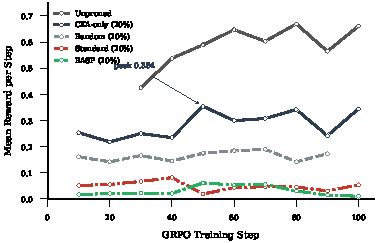
\includegraphics[width=\columnwidth]{figures/paper/fig2_reward_trajectories.pdf}
    \caption{GRPO reward trajectories for four pruning criteria under identical training configuration ($\beta{=}0.01$, $T{=}0.4$, 100 steps). CKA-only (blue) reaches 0.354 peak reward with sustained improvement and self-recovery from a step-90 perturbation. Random (orange) oscillates between 0.14 and 0.19 without learning. Standard (vermillion) peaks at 0.081 before borderline collapse. \rasp{} (reddish purple) peaks at 0.061 and collapses irreversibly by step 50. Grey dashed line: unpruned model (0.669 peak).}
    \label{fig:reward_trajectories}
\end{figure}

The central finding of this work is that the pruning criterion determines post-RLVR recovery capacity.
Under controlled GRPO training with identical hyperparameters, the four pruning methods produce qualitatively distinct training dynamics that form a clear recovery capacity gradient: CKA-only $\gg$ Random $\gg$ Standard $>$ \rasp{}.
Table~\ref{tab:recovery_gradient} summarizes the key metrics, and Figure~\ref{fig:reward_trajectories} shows the reward trajectories over 100 GRPO steps.

CKA-only pruning is the only method that produces active learning under GRPO.
Reward reaches a peak of 0.354 with mean 0.275 across training.
The fraction of training batches with zero reward standard deviation ($f_0$, a proxy for policy collapse where all sampled completions receive identical reward and produce no learning signal) reaches a minimum of 0.125 at step 70, indicating healthy exploration.
At step 90, the model experiences a transient perturbation ($f_0$ spikes to 0.300), but it self-recovers to reward 0.344 by step 100.
This self-recovery capacity is unique among the four methods and indicates that the retained architecture contains sufficient functional diversity to escape local policy degeneration.
Random pruning produces stagnation: reward oscillates between 0.142 and 0.190 across 90 steps (mean 0.164) with no sustained improvement, while $f_0$ holds steady between 0.300 and 0.350.
The model generates diverse completions but cannot convert exploration into reward gain.

\begin{figure}[t]
    \centering
    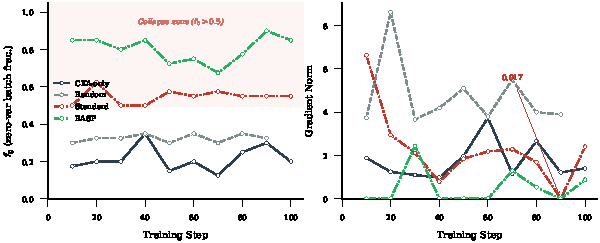
\includegraphics[width=\columnwidth]{figures/paper/fig3_collapse_dynamics.pdf}
    \caption{Collapse dynamics measured by $f_0$ (fraction of training batches where all sampled completions receive identical reward). CKA-only (blue) stays below 0.30 throughout training. Random (orange) holds near 0.33. Standard (vermillion) starts at 0.50 and remains elevated. \rasp{} (reddish purple) climbs monotonically from 0.675 to 0.850, indicating progressive and irreversible policy collapse.}
    \label{fig:collapse_dynamics}
\end{figure}

Standard pruning exhibits borderline collapse (Figure~\ref{fig:collapse_dynamics}).
Reward peaks at 0.081 (step 40), then oscillates near 0.05 for the remaining steps (mean 0.050).
$f_0$ starts at 0.500 and stays between 0.500 and 0.625, so more than half of training batches produce no learning signal.
Gradient norm drops to 0.017, leaving minimal capacity for policy updates.
\rasp{} pruning produces the most severe outcome: full and irreversible collapse.
Reward peaks at 0.061 (step 20), falls to 0.010 by step 50, and remains there for the rest of training.
$f_0$ climbs monotonically from 0.675 to 0.850, meaning that in 85\% of training batches every sampled completion receives the same zero reward.
The model degenerates into repetitive token sequences with no gradient signal to escape.

The 5.8$\times$ gap in peak reward between CKA-only (0.354) and \rasp{} (0.061), and the 14.5$\times$ gap in mean reward (0.275 vs 0.019), arise from models pruned to identical parameter budgets and trained with identical GRPO configurations.
The only variable is which structures were removed.
This isolation establishes that recovery capacity is a direct function of the pruning criterion.
For reference, the unpruned model achieves 0.669 peak reward with stable training across all 100 steps ($f_0 < 0.275$), placing the best pruned result (CKA-only) at 53\% of unpruned recovery capacity.


\subsection{Reward-Accuracy Decoupling}
\label{sec:decoupling}

\input{tables/tab2_decoupling}

Table~\ref{tab:decoupling} compares SFT accuracy with GRPO accuracy on the full test set ($N{=}1{,}319$, greedy decoding).
Across all evaluated configurations, GRPO training increases reward but does not improve reasoning accuracy.
The unpruned model achieves 81.27\% after SFT and an identical 81.27\% after 100 GRPO steps (1{,}072 of 1{,}319 problems yield the same correct answer at both stages), despite reward rising from 0 to 0.669.
Standard-pruned accuracy drops by 0.38 percentage points (pp) from SFT (59.29\%) to the last stable GRPO checkpoint at step 50 (58.91\%).
\rasp{}-pruned accuracy drops by 0.84\,pp from SFT (61.49\%) to step 5 (60.65\%).
No configuration shows accuracy improvement from GRPO.

The decoupling is bidirectional: reward increases do not produce accuracy gains, and reward collapse does not produce proportional accuracy losses.
The Standard model's reward drops from peak 0.081 to 0.019 at step 50 (a 4$\times$ decline), yet accuracy at step 50 decreases by only 0.38\,pp relative to SFT.
Under GSM8K's binary reward with greedy decoding, GRPO's learning signal appears to capture formatting or stylistic properties of the generation rather than reasoning correctness.


\subsection{SFT Recovery Gradient}
\label{sec:sft_gradient}

Under SFT recovery alone ($N{=}1{,}319$), the three evaluated methods produce a gradient that partially differs from the GRPO ranking: CKA-only (63.91\%) $>$ \rasp{} (61.49\%) $>$ Standard (59.29\%).
CKA-only leads both rankings, confirming that redundancy-based pruning preserves the best recovery substrate regardless of the downstream paradigm.
The advantage of \rasp{} over Standard (+2.20\,pp) is consistent with the design rationale: the CKA overlap penalty removes structures whose function overlaps with retained peers, and teacher-forced gradient updates can redistribute computation across those peers.
The gap between CKA-only and \rasp{} (+2.42\,pp) indicates that gradient importance weighting in the composite score (Eq.~\ref{eq:score}) harms SFT recovery relative to pure redundancy-based selection.

The critical divergence between the SFT and GRPO rankings appears in the bottom half.
Under SFT, \rasp{} (61.49\%) outperforms Standard (59.29\%).
Under GRPO, the ordering reverses: Standard reaches 0.081 peak reward while \rasp{} peaks at only 0.061 before full collapse.
The CKA component in \rasp{} preferentially removes redundant structures, which are safely removable under teacher forcing but provide exploration stability that GRPO requires.
CKA-only avoids this failure because it removes redundant structures without also deprioritizing important ones through the composite score.


\subsection{Sparsity Cliff at 30\%}
\label{sec:sparsity_cliff}

\input{tables/table4_sparsity_cliff}

Table~\ref{tab:sparsity_cliff} reports accuracy at 30\% sparsity ($N{=}100$).
All three tested methods collapse: Standard retains only 4\% accuracy with 5.5\% EOS generation rate, \rasp{} drops to 0\% with 3.0\% EOS rate, and CKA-only also reaches 0\% (experiment terminated early after collapse confirmed).
This universal failure at 30\% sparsity, independent of pruning criterion, indicates a structural capacity threshold beyond which no selection strategy preserves sufficient reasoning capacity.
The cliff validates 20\% as the operating point for the main experiments and suggests that the recovery capacity gradient at 20\% reflects how methods allocate a limited pruning budget, not differences in total capacity preservation.


\subsection{Inference Efficiency}
\label{sec:inference}

\input{tables/table5_inference}

Table~\ref{tab:inference} reports inference latency and GPU memory at 20\% sparsity.
\rasp{}-pruned models achieve 37.8\% latency reduction (6.682\,s to 4.156\,s), compared to 7.7\% for Standard (6.682\,s to 6.167\,s).
Both achieve comparable memory savings (28.5\% vs 28.4\%), as expected from identical parameter counts.
The 4.9$\times$ latency gap arises because \rasp{}'s CKA-aware selection produces more uniform layer-wise sparsity, allowing more layers to benefit from reduced MLP width.
Standard pruning concentrates removal in globally low-importance layers, leaving bottleneck layers at full width that limit throughput.


\subsection{Ablation: CKA Coefficient $\alpha$}
\label{sec:ablation}

\begin{table}[t]
\centering
\caption{Ablation over the CKA balancing coefficient $\alpha$ at 20\% sparsity. $\alpha{=}0$ reduces to standard importance-only pruning; higher $\alpha$ increases the weight of CKA-based representational similarity in head selection.}
\label{tab:alpha}
\begin{tabular}{S[table-format=1.1] S[table-format=2.0] l l}
\toprule
{$\alpha$} & {Post-Prune Acc (\%)} & {CKA Weight} & {Interpretation} \\
\midrule
0.0 & 1                      & None         & $=$ Standard pruning \\
0.5 & \textcolor{gray}{TBD} & Low          & Slight CKA awareness \\
1.0 & 29                     & Medium       & Default RASP \\
2.0 & \textcolor{gray}{TBD} & High         & Strong CKA emphasis \\
4.0 & \textcolor{gray}{TBD} & Very High    & Dominant CKA weight \\
\bottomrule
\end{tabular}
\end{table}


Table~\ref{tab:alpha} reports post-prune accuracy across $\alpha \in \{0.0, 0.25, 0.5, 1.0, 2.0\}$ at 20\% sparsity ($N{=}100$).
At $\alpha{=}0.0$ (Standard pruning), accuracy is 27\%.
Accuracy initially decreases to 22\% at $\alpha{=}0.5$, then increases monotonically to 36\% at $\alpha{=}2.0$.
The initial dip at intermediate $\alpha$ reflects a transition region where importance and redundancy signals partially cancel: the pruner avoids both low-importance structures (protected by $I(h)$) and redundant structures (protected by $(1-F(h))^\alpha$), removing instead structures that are moderately important and moderately unique.
This combination is the worst for capacity preservation.

At $\alpha{=}0.0$, post-SFT accuracy reaches 64\% ($N{=}100$), the highest observed value despite lower post-prune accuracy (27\%).
This reversal reinforces the SFT recovery gradient (Section~\ref{sec:sft_gradient}): the architecture that best survives pruning is not the best substrate for SFT recovery.
Low-$\alpha$ configurations retain individually important structures that teacher forcing exploits effectively.


\subsection{Discussion}
\label{sec:discussion}

The recovery capacity gradient reveals a counterintuitive finding: gradient-based importance scoring, the standard criterion for structured pruning~\citep{llmpruner2023}, is a harmful signal for RLVR recovery.
Methods that use Taylor-expansion importance (Standard and \rasp{}) produce the two worst GRPO outcomes, while CKA-only (no importance signal) achieves the best recovery and Random pruning outperforms both importance-based methods.

Taylor-expansion importance $I(h)$ identifies structures whose removal causes the largest immediate output perturbation.
Standard pruning removes the ``least important'' structures, preserving the primary reasoning pathways but eliminating backup computational paths that are currently inactive yet available for exploration.
GRPO pushes the model toward unfamiliar output distributions, and these backup paths provide the capacity to explore new reasoning strategies.
When they are absent, the policy converges to a degenerate fixed point from which it cannot escape (Section~\ref{sec:recovery_gradient}).

CKA-only pruning removes structures with the highest functional overlap among within-layer peers.
This preserves all functionally unique computational paths, including currently inactive ones, yielding maximum functional diversity in the retained architecture.
The self-recovery at step 90 is a direct consequence: even after a perturbation collapses part of the policy, alternative computational paths remain available to reconstruct coherent generation.
Random pruning outperforms importance-based methods because it does not systematically target any structural category, preserving a representative sample of the architecture's functional diversity by chance.

These results suggest that pruning criteria should be evaluated not by immediate accuracy retention but by the downstream recovery capacity they enable.
For RLVR recovery, functional diversity measured by CKA overlap is a more informative pruning criterion than gradient importance.
CKA-only pruning, the simplest method in our comparison (forward-pass CKA computation only, no gradient collection needed), produces both the best RLVR recovery and the best SFT recovery.
